\subsection{\acs{owasp}}

\acs{owasp} ist das Akronym für \textbf{O}pen \textbf{W}eb
\textbf{A}pplication \textbf{S}ecurity \textbf{P}roject und
beschreibt eine offene Organisation, deren Hauptziel ist, die
Sicherheit von Anwendungen, Diensten und Software zu verbessern.
Sie wurde am 1. Dezember 2001 gegründet und am 21. April 2004 als
gemeinnützige Organisation offiziell anerkannt.  Sie ermöglicht
Organisationen, Unternehmen oder Einzelpersonen, sichere Anwendungen zu
entwickeln und zu warten. Die \acs{owasp} hat eine Reihe von
Sicherheitstools und -richtlinien entwickelt. Dazu gehören die \acs{owasp}
Top 10 und der Zed Attack Proxy (\acs{zap}). Ein wichtiger
Grundsatz der OWASP ist, dass jeder, der sich für die Sicherheit
von Webanwendungen interessiert, weltweit kostenlos über das
nötige Wissen und die Werkzeuge verfügen kann (vgl. \cite{owasp}).
In diesem Zusammenhang hat sie die OWASP TOP 10 erstellt, die eine
Liste der zehn häufigsten Sicherheitslücken im Internet
darstellt. Ihr Hauptzweck ist die Schulung all jener, die mit der
Entwicklung sicherer Anwendungen zu tun haben.  Sie sollen über die
üblichsten Sicherheitslücken informiert werden und dadurch diese
vermeiden.  Im Folgenden werden die zehn Angriffe der OWASP TOP
10 auf der Basis der OWASP TOP 10 2017 
Release Candidate 2 (vgl. \cite{Stock2017}) beschrieben.

\begin{table}[h]
    \begin{tabulary}{\textwidth}{@{}L@{}}
        \toprule
        \textbf{OWASP TOP10 2017} \tabularnewline\midrule
        1"~ Injektion (Injection)
        \tabularnewline
        2"~ Fehler in der Authentifizierung (Broken Authentication)
        \tabularnewline
        3"~ Verlust der Vertraulichkeit von Daten (Sensitive Data Exposure)
        \tabularnewline
        4"~ XML External Entities (XML)
        \tabularnewline
        5"~ Fehler in der Zugriffskontrolle (Broken Access Control)
        \tabularnewline
        6"~ Sicherheitsrelevante Fehlkonfiguration (Security Misconfiguration)
        \tabularnewline
        7"~ Cross-Site-Scripting (XSS)
        \tabularnewline
        8"~ Unsichere Deserialisierung (Insecure Deserialization)
        \tabularnewline
        9"~ Nutzung von Komponenten mit bekannten Schwachstellen (Using Components with Known Vulnerabilities)
        \tabularnewline
        10"~ Unzureichendes Logging und Monitoring (Insufficient Logging and Monitoring)
        \tabularnewline\bottomrule
    \end{tabulary}
    \caption{OWASP TOP 10 2017}\label{tab:OWASP_TOP_10}
\end{table}

\subsubsection{Injektion}

Eine Injektion ist eine Schwachstelle, die einem Angreifer ermöglicht,
bösartigen Code durch eine Anwendung auf ein anderes System zu
schleusen. Dabei können sowohl Backend-Systeme als auch andere
Clients, die mit der angreifbaren Anwendung verbunden sind, gefährdet
werden. Zu den Auswirkungen dieser Angriffe gehören:

\begin{enumerate}
    \item Einem Angreifer erlauben, Betriebssystemaufrufe auf einem
    Zielrechner auszuführen.
    \item Einem Angreifer ermöglichen, Backend-Datenspeicher
    zu kompromittieren.
    \item Einem Angreifer ermöglichen, die Sitzungen anderer
    Benutzer zu kompromittieren oder umzuleiten.
    \item Einem Angreifer erlauben, Aktionen im Namen anderer
    Benutzer oder Dienste zu erzwingen.
\end{enumerate}

Viele Webanwendungen hängen von Betriebssystemfunktionen, externen
Programmen und der Verarbeitung von Datenabfragen ab, die von
Benutzern eingereicht werden. Wenn eine Webanwendung Informationen
aus einer HTTP-Anfrage als Teil einer externen Anfrage weitergibt,
sollten Sie eine Möglichkeit zur Überprüfung und Validierung der
Nachricht einrichten. Andernfalls kann ein Angreifer spezielle
(Meta-) Zeichen, bösartige Befehle/Codes oder Befehlsmodifikatoren in
die Nachricht einfügen. Diese Angriffe sind zwar nicht schwer
auszuführen, aber es gibt immer mehr Tools, die nach diesen
Fehlern suchen. Ein Angreifer kann diese Techniken nutzen, um den
Inhalt Ihrer Datenbank zu erhalten, zu beschädigen oder zu zerstören,
Backend-Systeme zu kompromittieren oder andere Benutzer anzugreifen.
Erfolgreiche Injektionsangriffe können ein System vollständig
gefährden oder zerstören. Es ist wichtig, auf diese Arten von
Angriffen zu testen und sich dagegen zu schützen.

Als Beispiel kann man die SQL-Injektion nennen. Diese ist eine
besonders weit verbreitete und gefährliche Form der Injektion.
Um einen SQL-Injektion-Fehler auszunutzen, muss ein Angreifer
einen Parameter finden, den die Webanwendung an eine
Datenbankinteraktion weitergibt. Ein Angreifer kann dann
bösartige SQL-Befehle in den Inhalt des Parameters einbetten.
Das bringt die Webanwendung dazu, eine bösartige Abfrage an die
Datenbank weiterzuleiten. SQL-Abfragen könnten durch Hinzufügen
zusätzlicher ``Einschränkungen'' zu einer Anweisung (z. B. OR 1=1)
geändert werden, um Zugriff auf nicht autorisierte Daten zu
erhalten oder diese zu ändern.



\subsubsection{Fehler in der Authentifizierung}

Wenn die Authentifizierungsfunktionen  einer Anwendung nicht korrekt
implementiert sind, können Angreifer Passwörter oder Sitzungs-IDs
kompromittieren oder andere Implementierungsfehler ausnutzen, indem
sie die Anmeldedaten anderer Benutzer verwenden. Diese Schwachstelle
wird als ``Fehler in der Authentifizierung'' (Broken authentication
in Englisch) bezeichnet. Es wird in der Regel durch schlecht
implementierte Authentifizierungs- und Sitzungsverwaltungsfunktionen
verursacht. In diesem Fall  zielen Angriffe darauf ab, die Kontrolle
über ein oder mehrere Benutzerkonten zu erlangen, indem der Angreifer
die gleichen Privilegien erhält wie der angegriffene Benutzer.
Es wird vom ``Fehler in der Authentifizierung'' besprochen ,
wenn Angreifer in der Lage sind, Passwörter, Schlüssel oder
Sitzungs-Tokens, Benutzerkontoinformationen und andere
Details zu kompromittieren, um Benutzeridentitäten zu übernehmen.
Zu den üblichen Risikofaktoren gehören:


\begin{enumerate}
    \item Vorhersehbare Anmeldekennungen
    \item Benutzerauthentifizierungskennungen, die nicht geschützt sind, wenn sie gespeichert werden.
    \item Sitzungs-IDs, die in der URL offengelegt werden (z. B. durch URL-Rewriting).
    \item Sitzungs-IDs, die anfällig für Session-Fixing-Angriffe sind.
    \item Sitzungswert, der nach dem Abmelden nicht unterbrochen oder ungültig gemacht wird.
    \item Sitzungskennungen, die nach einer erfolgreichen Anmeldung nicht erneuert werden.
    \item Passwörter, Sitzungskennungen und andere Identifikationsinformationen, die über unverschlüsselte Verbindungen gesendet werden.
\end{enumerate}
\subsubsection{Verlust der Vertraulichkeit von Daten}

Der Verlust der Vertraulichkeit von  Daten tritt auf, wenn eine
Organisation unwissentlich sensible Daten offenlegt oder wenn ein
Sicherheitsvorfall dazu führt, dass sensible Daten versehentlich
oder rechtswidrig zerstört, verloren, verändert, unbefugt
offengelegt oder unbefugt darauf zugegriffen wird. Eine solche
Datenexposition kann das Ergebnis eines unzureichenden Schutzes einer
Datenbank, einer Fehlkonfiguration bei der Erstellung neuer Instanzen
von Datenspeichern oder einer unsachgemäßen Nutzung von Datensystemen sein.

Klassische Beispiele dafür sind in Klartext gespeicherte Daten, wie
Passwörter oder Kreditkartendaten, fehlendes HTTPS auf
authentifizierten Webseiten, und Hash-Passwörter, die ohne zugefügtes
“Salz” erstellt wurden. Salz bezeichnet eine zufällige Zeichenfolge,
die den Klardaten vor der Verschlüsselung hinzugefügt werden. Dadurch
kann anhand identischer Hashwerte nicht darauf geschlossen werden,
dass es sich um dieselben Daten handelt.
\subsubsection{XML External Entities (XML)}

\acs{xml} External Entity Injection (auch bekannt als \acs{xee}) ist eine
Sicherheitslücke, die einem Angreifer ermöglicht, in die Verarbeitung
von \acs{xml}-Daten durch eine Anwendung einzugreifen. Dieser Angriff
erfolgt, wenn die \acs{xml}-Eingabe, die einen Verweis auf eine externe
Entität enthält, von einem schwach konfigurierten \acs{xml}-Parser
verarbeitet wird. Dieser Angriff kann zur Offenlegung vertraulicher
Daten, Denial of Service, serverseitiger Anfragefälschung,
Portanalyse aus der Sicht des Computers, auf dem sich der Parser
befindet, und anderen Auswirkungen auf das System führen. Um \acs{xxe}
Injections zu verhindern, sollen folgende Punkte beachtet werden:


\begin{enumerate}
    \item Einfachere Datenformate wie JSON zur Datenübertragung verwenden.
    \item Das Verbot in allen \acs{xml}-Parsern, \acs{xml}-Entitäten
     und \acs{dtd}s verändern. \acs{dtd} steht für Document Type Definition und
     bezeichnet einen XML Dokument, in welchem XML-Entities
     definiert werden. Auf dieser Weise wird vermieden,
     dass ein Benutzer eigenen Entities erstellt.
    \item Deaktivierung des Hochladens von XML-Dateien
\end{enumerate}

\subsubsection{Fehler in der Zugriffskontrolle}

Fehler in der Zugriffskontrolle ist eine Sicherheitslücke,
die es Angreifern ermöglicht, Berechtigungsgarantien zu
umgehen und Tätigkeiten auszuführen, als wären sie
privilegierte Benutzer.

Die Zugriffskontrolle sorgt dafür, dass Benutzer nicht
außerhalb der ihnen zugewiesenen Befugnisse handeln
können. Fehler führen in der Regel zur unbefugten
Offenlegung von Informationen, zur Änderung oder Zerstörung
aller Daten oder zur Ausführung einer Geschäftsfunktion
außerhalb der Grenzen des Benutzers. Häufige Schwachstellen
bei der Zugriffskontrolle sind:

\begin{enumerate}
    \item Umgehung von Zugriffskontrollprüfungen durch
    Änderung der URL, des internen Anwendungsstatus oder
    der HTML-Seite oder einfach durch Verwendung eines
    benutzerdefinierten API-Angriffstools.

    \item Ermöglichung der Änderung des Primärschlüssels
    in den Datensatz eines anderen Benutzers, wodurch
    die Anzeige oder Bearbeitung des Kontos eines anderen
    Benutzers ermöglicht wird.

    \item Ausweitung der Rechte. Als Benutzer handeln, ohne
    eingeloggt zu sein, oder als Administrator handeln, wenn
    man als Benutzer eingeloggt ist.

    \item Manipulation von Metadaten, wie z. B. die
    Wiedergabe oder Manipulation eines JSON Web Token
    (JWT)-Zugangskontrolltokens oder eines Cookies oder
    eines versteckten Feldes, das manipuliert wurde, um
    die Privilegien zu erhöhen, oder der Missbrauch der
    JWT-Ungültigkeitserklärung.

    \item CORS-Fehlkonfiguration ermöglicht
    nicht autorisierten API-Zugriff.

    \item Erzwingen des Navigierens auf authentifizierten
    Seiten als nicht authentifizierter Benutzer oder
    auf privilegierten Seiten als Standardbenutzer.
    Zugriff auf API mit fehlenden Zugriffskontrollen
    für POST, PUT und DELETE.
\end{enumerate}

\subsubsection{Sicherheitsrelevante Fehlkonfiguration}

Sicherheitsrelevante Fehlkonfigurationen sind 
Sicherheitskontrollen, die ungenau konfiguriert oder
unsicher sind. Dadurch werden Ihre Systeme und Daten 
gef\"ahrdet. Grunds\"atzlich kann jede schlecht dokumentierte 
Konfigurations\"anderung, Standardeinstellung oder ein 
technisches Problem bei einer beliebigen Komponente zu 
einer Fehlkonfiguration f\"uhren.

Eine Fehlkonfiguration kann aus einer Vielzahl von 
Gr\"unden auftreten. Moderne Netzwerkinfrastrukturen sind
\"au{\ss}erst komplex und zeichnen sich durch st\"andige
Ver\"anderungen aus. Organisationen k\"onnen leicht 
entscheidende Sicherheitseinstellungen \"ubersehen, 
insbesondere bei neuen Netzwerkger\"aten, die 
Standardkonfigurationen beibehalten k\"onnen. Wenn
sichere Konfigurationen f\"ur Zugangspunkte eingerichtet 
werden, m\"ussen Konfigurationen mit Sicherheitskontrollen
h\"aufig \"uberpr\"uft werden, um unvermeidliche 
Konfigurationsabweichungen zu erkennen. Systeme
\"andern sich, neue Ger\"ate werden in das Netzwerk
eingef\"uhrt, Patches werden eingespielt - all dies
tr\"agt zu fehlerhaften Konfigurationen bei.


\subsubsection{Cross-Site-Scripting (XSS)}
\subsubsection{Unsichere Deserialisierung}

Der Begriff Serialisierung stammt aus der objektorientierten
Programmierung und bezeichnet die Umwandlung eines programmierten
Objekts (z. B. ein Java-, Python-Objekt) in eine Folge von Bytes.
Die Serialisierung sorgt dafür, dass erstellte Objekte nicht nur zur
Laufzeit, sondern auch danach existieren. Es ist daher eine Methode,
die für die Persistenz von Objekten verwendet wird. Sie wird auch
verwendet, um Objekte über ein Netzwerk zu übertragen (vgl. \cite{serial}).
Die Deserialisierung ist der umgekehrte Prozess der Serialisierung und
erzeugt wieder ein Objekt aus einem Bytestream.

\begin{figure}[H]
    \centering
    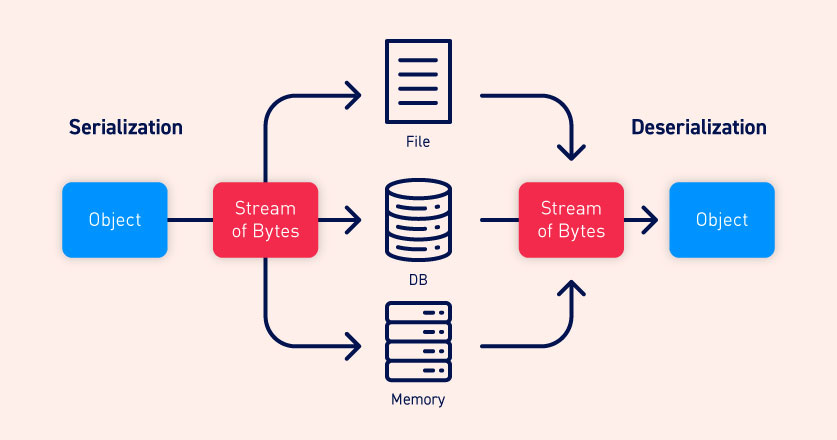
\includegraphics[scale=0.4]{images/deserialization-diagram}
    \caption{Deserialisierung Diagram (vgl. \cite{deserial-img})} \label{fig:des}
\end{figure}

Eine unsichere Deserialisierung liegt vor, wenn vom Benutzer kontrollierbare
Daten von einer Website deserialisiert werden. Dies ermöglicht es einem
Angreifer potenziell, die serialisierten Objekte zu manipulieren, um
schädliche Daten in den Anwendungscode einzuschleusen. Es ist sogar
möglich, ein serialisiertes Objekt durch ein Objekt einer völlig anderen
Klasse zu ersetzen. Alarmierenderweise werden Objekte jeder beliebigen
auf der Website verfügbaren Klasse deserialisiert und instanziiert,
unabhängig von der erwarteten Klasse. Aus diesem Grund wird die unsichere
Deserialisierung manchmal auch als "Objektinjektions"-Schwachstelle
bezeichnet  (vgl. \cite{deserial-img}).

Ein Objekt einer unerwarteten Klasse kann eine Ausnahme auslösen.
Zu diesem Zeitpunkt kann der Schaden jedoch bereits eingetreten sein.
Viele Angriffe, die auf Deserialisierung basieren, werden durchgeführt,
bevor die Deserialisierung abgeschlossen ist. Das bedeutet, dass der
Prozess der Deserialisierung selbst einen Angriff auslösen kann, auch
wenn die eigentliche Funktionalität der Website nicht direkt mit dem
bösartigen Objekt interagiert. Aus diesem Grund können auch Webseiten,
deren Logik auf stark typisierten Sprachen basiert, für diese Techniken
anfällig sein  (vgl. \cite{deserial-img}).

\subsubsection{Nutzung von Komponenten mit bekannten Schwachstellen}
\subsubsection{Unzureichendes Logging und Monitoring}

Protokolle (Logs) geben Einblick in die Aktivit\"aten einer
Organisation. Die erstellten Protokolle und Pr\"ufpfade 
erm\"oglichen einer Organisation die Fehlerbehebung, die Verfolgung von
Ereignissen, die Erkennung von Zwischenf\"allen und die Einhaltung
gesetzlicher Vorschriften. Unzureichende Protokollierung und \"uberwachung 
bedeutet, dass sicherheitskritische Informationen nicht protokolliert
werden oder dass das richtige Protokollformat, der richtige Kontext,
die richtige Speicherung, die richtige Sicherheit und eine rechtzeitige
Reaktion fehlen, um einen Vorfall oder eine Sicherheitsverletzung zu 
erkennen.

Laut dem IBM-Bericht \"uber Datenschutzverletzungen aus dem Jahr 2020 dauert
es durchschnittlich 280 Tage, bis eine Datenschutzverletzung entdeckt und
einged\"ammt wird (vgl. \cite{ibm-sec}, S. 11). Protokolle sind ein wichtiger
Bestandteil der Reaktion auf Vorf\"alle. Ein Unternehmen kann von einer 
Sicherheitsverletzung \"uberrascht werden, die unentdeckt bleiben kann 
und irreparable rechtliche, finanzielle und regulatorische Folgen 
haben kann. Eine ordnungsgem\"a{\ss}e Protokollverwaltung sorgt f\"ur eine
schnellere Erkennung und Eind\"ammung von Sicherheitsverletzungen und
spart dem Unternehmen Zeit, Geld und Ansehen.

